\section{Pictogram Endpoint}\label{pictogramendpoint}
This section will solve the \userstory{As a developer i would like an endpoint for Pictograms, such that i can retrieve them from GIRAF.}

The Pictogram endpoint is used for the PictoSearch library to find different pictograms, as well as to get specific pictograms which have not been downloaded yet.
Currently in the PictoSearch library a user searches for some string, and the local database is queried using \texttt{... LIKE \%searchstring\%} and as such this will also be used for the REST API.
Therefore a goal of the REST API for pictograms is to provide a search method, such that PictoSearch will result in the same results as before.
The endpoint will also be used in the case that a user opens, e.g. a week schedule which contains a pictogram that the device have not saved locally, the endpoint will then retrieve this single pictogram rather than returning a list of pictograms.

The model that was described in \myref{restapimodel} was the complete model of the REST API \myref{fig:screenshot_newsearch} shows the model regarding pictograms along with the fields of these classes.

\begin{figure}[h]
    \centering
    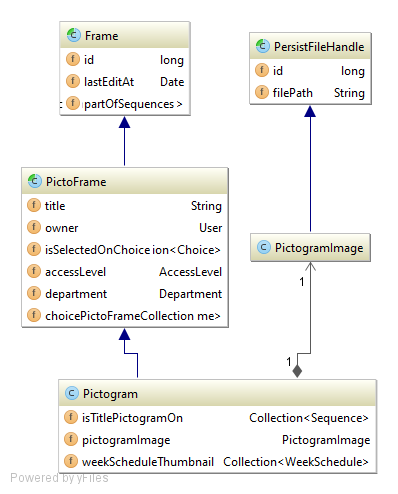
\includegraphics[width=0.5\textwidth]{figures/diagram-pictogram.png}
    \caption{Class-diagram including fields of the classes involved in Pictograms}\label{fig:screenshot_newsearch}
\end{figure}\todo{Update accordingly in the end}

Here a brief description of the purpose for each field of the classes on the figure will be given.
\subsubsection*{Frame}
	\begin{description}
		\item[id] This is the id of the Frame which is saved in the database.
		\item[lastEditAt] This is a time stamp of when the Frame was last edited. 
		It is to be used for conflict handling as e.g. pictograms can be altered in the PictoCreator tool, and a need for conflict handling is therefore needed.
		\item[partofSequences] This is a collection if sequences this frame is used in, and why this collection is here will be further explained in \todo[inline]{sequenceendpointref}
	\end{description}

\subsubsection*{PictoFrame}
	\begin{description}
		\item[title] Title of the \texttt{PictoFrame}, it is used to search for and also to show what the \texttt{PictoFrame} is called when shown with its title in different parts of GIRAF.
		\item[owner] The user which owns the \texttt{PictoFrame}. 
		This is used to accommodate the need for creating private \texttt{Pictograms} and \texttt{Sequences}.
		Private means that only the user who is owner can access them.
		\item[accessLevel] This is an Enumeration which specifies whether the \texttt{PictoFrame} is Public, shared on department or private.
		\item[department] Specifies which apartment the \texttt{PictoFrame} belongs to, and is used when the accessLevel is specified as shared on department.
		\item[optionOn] A collection of all \texttt{Choice}s which contain the \texttt{PictoFrame}.
		This is needed for hibernate to create the many-to-many relationship between \texttt{PictoFrame} and \texttt{Choice}, and will probably not be used for anything else.
	\end{description}

\subsubsection*{Pictogram}
	\begin{description}
		\item[isTitlePictogramOn] A collection of the \texttt{Sequence}s which this \texttt{Pictogram} is the titlePictogram of.
		\item[pictogramImage] A reference to the \texttt{Pictogram}'s \texttt{PictogramImage}
		\item [weekScheduleThumbnail] Much like the \texttt{isTitlePictogramOn} but this is for a collection of \texttt{WeekSchule}s instead.
	\end{description}

\subsubsection*{PictogramImage}
The \texttt{PictogramImage} has no fields of its own, but is used to indicate that the image is used for a \texttt{Pictogram} instead of e.g. a UserIcon.
It inherits fields for PersistFileHandle instead.

\subsubsection*{PersistFileHandle}
This class is what all images in GIRAF will inherit from, this means \texttt{Pictogram}s and also \texttt{UserIcon}s. 
Originally when we started working on the REST API for Pictogram the \texttt{PersistFileHandle} did not exist and all information on this class was saved directly on the \texttt{UserIcon} class.
Why and how this new generality is created will be explained in \todo{ref til sektionen}.
It contains the following fields:
	\begin{description}
		\item[id] This field is self explanatory.
		\item[filePath] A string of the path to the file which the class points to, for the \texttt{Pictogram} endpoint it will be a Pictogram.
	\end{description}